\chapter{DHCP Snooping}\label{dhcp-snooping}

WHAT IS DHCP SNOOPING?

\begin{itemize}
\tightlist
\item
  DHCP SNOOPING is a security feature of SWITCHES that is used to filter
  DHCP messages received on UNTRUSTED PORTS
\item
  DHCP SNOOPING only filters DHCP MESSAGES.

  \begin{itemize}
  \tightlist
  \item
    Non-DHCP MESSAGES are not affected
  \end{itemize}
\item
  All PORTS are UNTRUSTED, by DEFAULT

  \begin{itemize}
  \tightlist
  \item
    Usually UPLINK PORTS are configured as TRUSTED PORTS, and DOWNLINK
    PORTS remain UNTRUSTED
  \end{itemize}
\end{itemize}

\begin{figure}
\centering
\pandocbounded{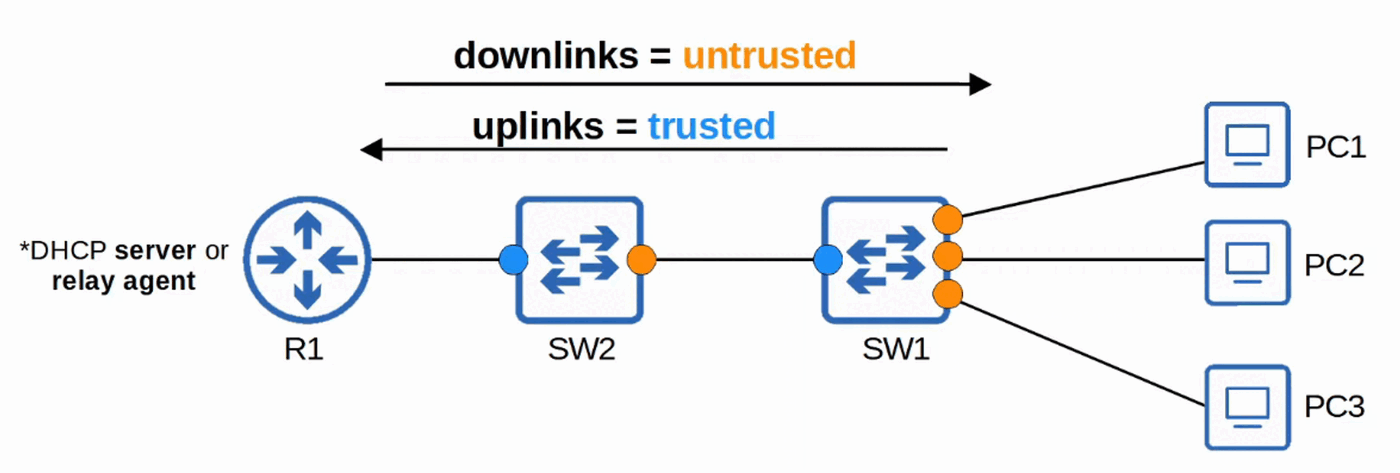
\includegraphics[keepaspectratio,alt={image}]{images/51-dhcp-snooping/img-001.png}}
\end{figure}

\begin{figure}
\centering
\pandocbounded{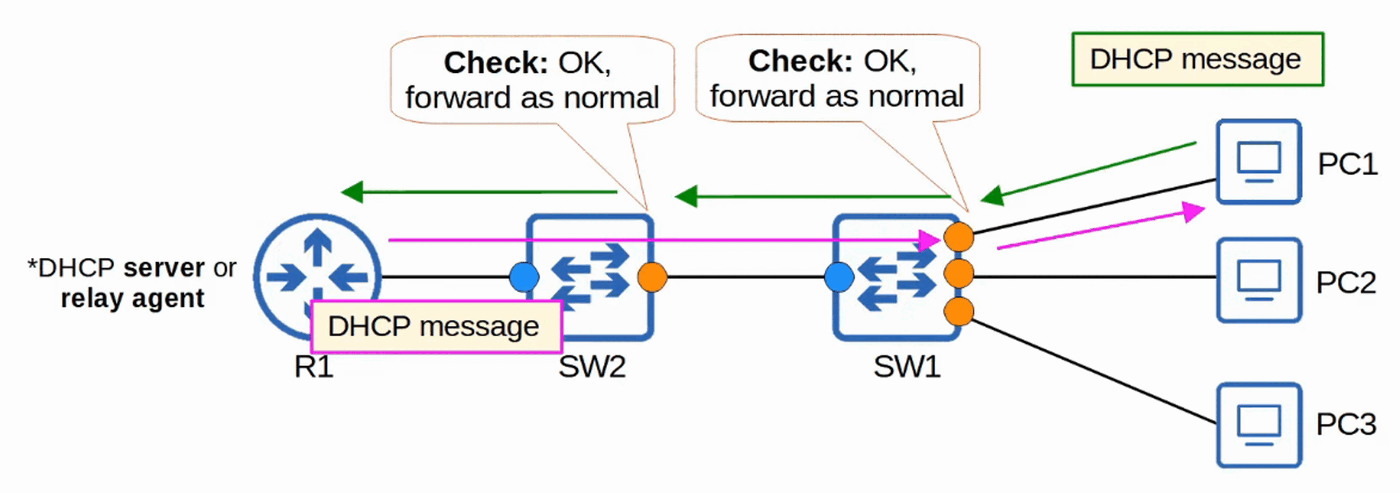
\includegraphics[keepaspectratio,alt={image}]{images/51-dhcp-snooping/img-002.png}}
\end{figure}

\section{Attacks on DHCP}\label{attacks-on-dhcp}

\section{DHCP Starvation}\label{dhcp-starvation}

\begin{itemize}
\tightlist
\item
  An example of a DHCP-based ATTACK is a DHCP STARVATION ATTACK
\item
  An ATTACKER uses spoofed MAC ADDRESSES to flood DHCP DISCOVER messages
\item
  The TARGET server's DHCP POOL becomes full, resulting in a DoS to
  other DEVICES
\end{itemize}

\begin{figure}
\centering
\pandocbounded{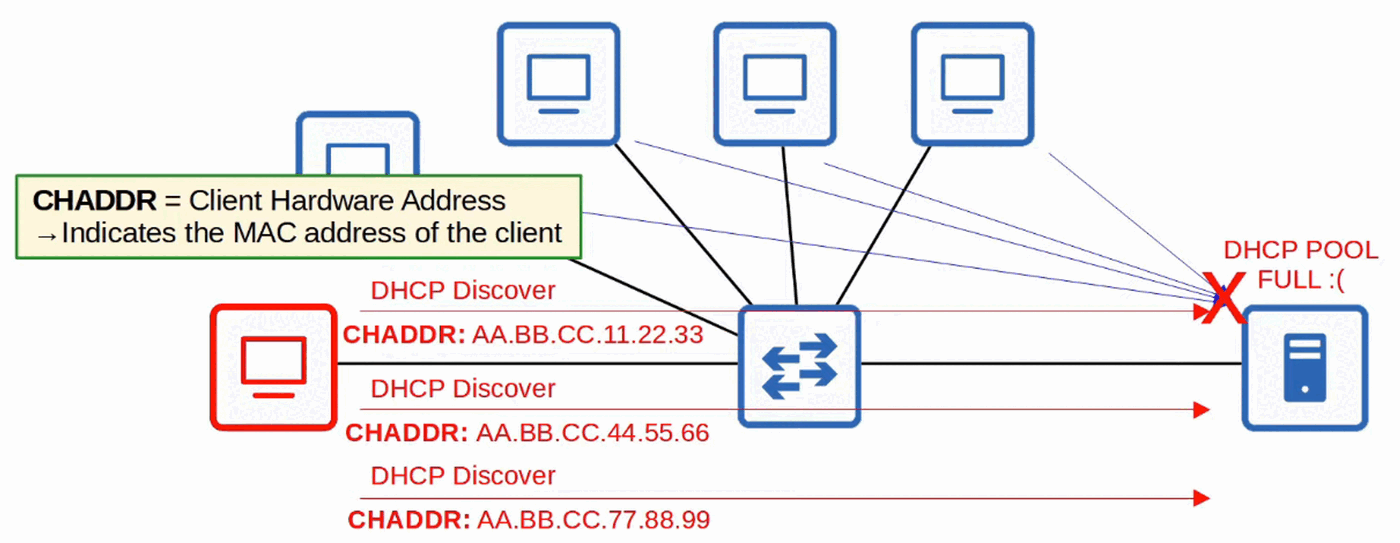
\includegraphics[keepaspectratio,alt={image}]{images/51-dhcp-snooping/img-003.png}}
\end{figure}

DHCP POISONING (Man-in-the-Middle)

\begin{itemize}
\tightlist
\item
  Similar to ARP POISONING, DHCP POISONING can be used to perform a
  Man-in-the-Middle ATTACK
\item
  A \emph{spurious DHCP SERVER} replies to CLIENTS' DHCP Discover
  messages and assigns them IP ADDRESSES but makes the CLIENTS use the
  \emph{spurious SERVER'S IP} as a DEFAULT GATEWAY
\end{itemize}

** CLIENTS usually accept the first DHCP OFFER message they receive

\begin{itemize}
\tightlist
\item
  This will cause the CLIENT to send TRAFFIC to the ATTACKER instead of
  the legitimate DEFAULT GATEWAY
\item
  The ATTACKER can then examine / modify the TRAFFIC before forwarding
  it to the legitimate DEFAULT GATEWAY
\end{itemize}

\begin{figure}
\centering
\pandocbounded{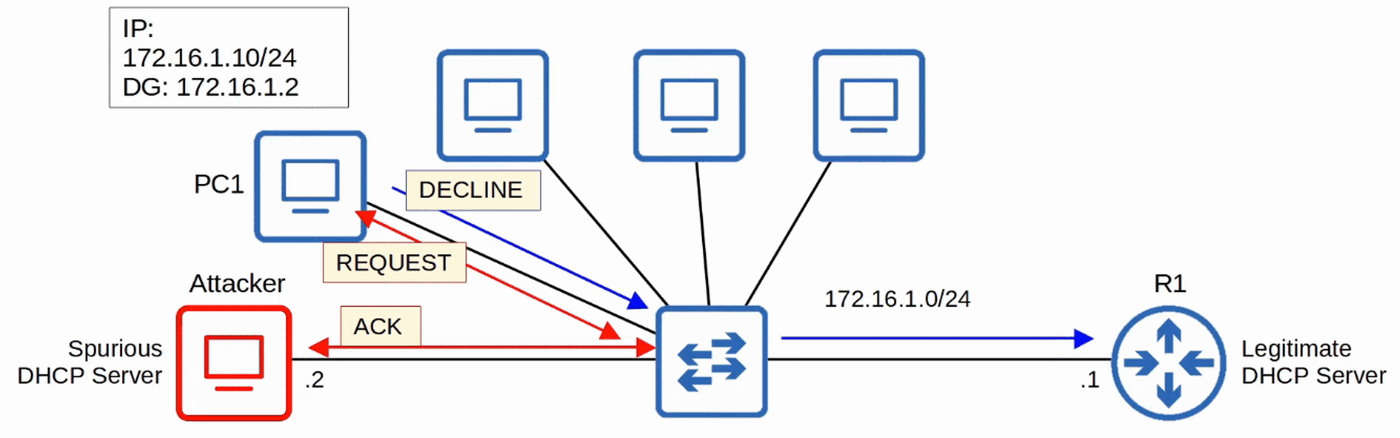
\includegraphics[keepaspectratio,alt={image}]{images/51-dhcp-snooping/img-004.png}}
\end{figure}

\begin{figure}
\centering
\pandocbounded{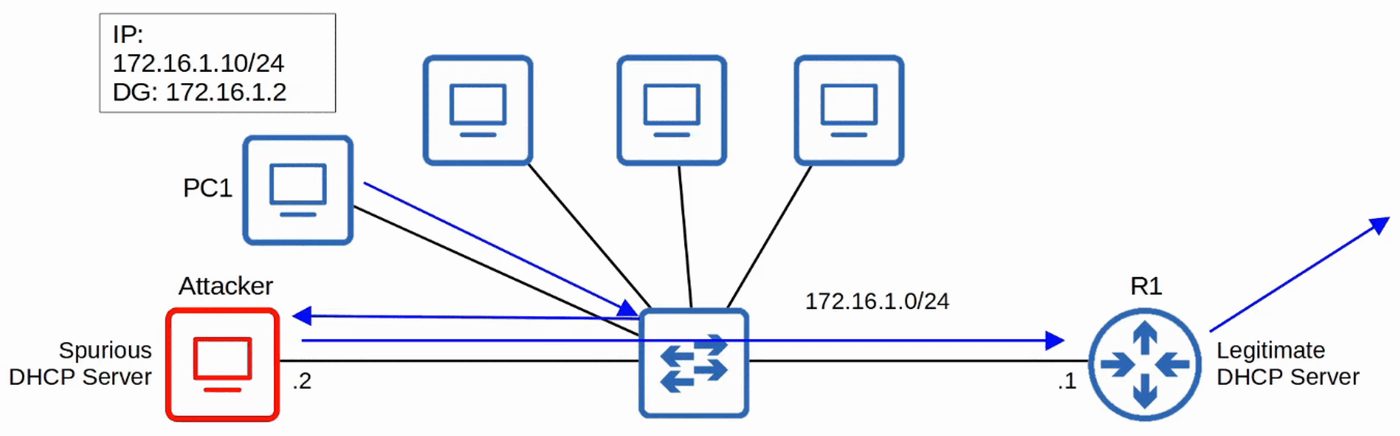
\includegraphics[keepaspectratio,alt={image}]{images/51-dhcp-snooping/img-005.png}}
\end{figure}

\section{DHCP Messages}\label{dhcp-messages}

\begin{itemize}
\item
  When DHCP SNOOPING filters messages, it differentiates between DHCP
  SERVER messages and DHCP CLIENT messages
\item
  Messages sent by DHCP SERVERS:

  \begin{itemize}
  \tightlist
  \item
    OFFER
  \item
    ACK
  \item
    NAK = Opposite of ACK - used to DECLINE a CLIENT'S REQUEST
  \end{itemize}
\item
  Messages sent by DHCP CLIENTS:

  \begin{itemize}
  \tightlist
  \item
    DISCOVER
  \item
    REQUEST
  \item
    RELEASE = Used to tell the SERVER that the CLIENT no longer needs
    its IP ADDRESS
  \item
    DECLINE = Used to DECLINE the IP ADDRESS offered by a DHCP SERVER
  \end{itemize}
\end{itemize}

HOW DOES IT WORK?

\begin{itemize}
\tightlist
\item
  If a DHCP MESSAGE is received on a TRUSTED PORT, forward it as normal
  without inspection
\item
  If a DHCP MESSAGE is received on an UNTRUSTED PORT, inspect it and act
  as follows:

  \begin{itemize}
  \tightlist
  \item
    If it is a DHCP SERVER message, discard it
  \item
    If it as a DHCP CLIENT message, perform the following checks:

    \begin{itemize}
    \tightlist
    \item
      DISCOVER / REQUEST messages :

      \begin{itemize}
      \tightlist
      \item
        Check if the FRAME'S SOURCE MAC ADDRESS and the DHCP MESSAGE'S
        CHADDR FIELDS match.

        \begin{itemize}
        \tightlist
        \item
          MATCH = FORWARD
        \item
          MISMATCH = DISCARD
        \end{itemize}
      \end{itemize}
    \item
      RELEASE / DECLINE messages:

      \begin{itemize}
      \tightlist
      \item
        Check if the PACKET'S SOURCE IP ADDRESS and the receiving
        INTERFACE match the entry in the \emph{DHCP SNOOPING BINDING
        TABLE}

        \begin{itemize}
        \tightlist
        \item
          MATCH = FORWARD
        \item
          MISMATCH = DISCARD
        \end{itemize}
      \end{itemize}
    \end{itemize}
  \end{itemize}
\item
  When a CLIENT successfully leases an IP ADDRESS from a SERVER, create
  a new entry in the \emph{DHCP SNOOPING BINDING TABLE}
\end{itemize}

\section{DHCP Snooping Configuration}\label{dhcp-snooping-configuration}

\begin{figure}
\centering
\pandocbounded{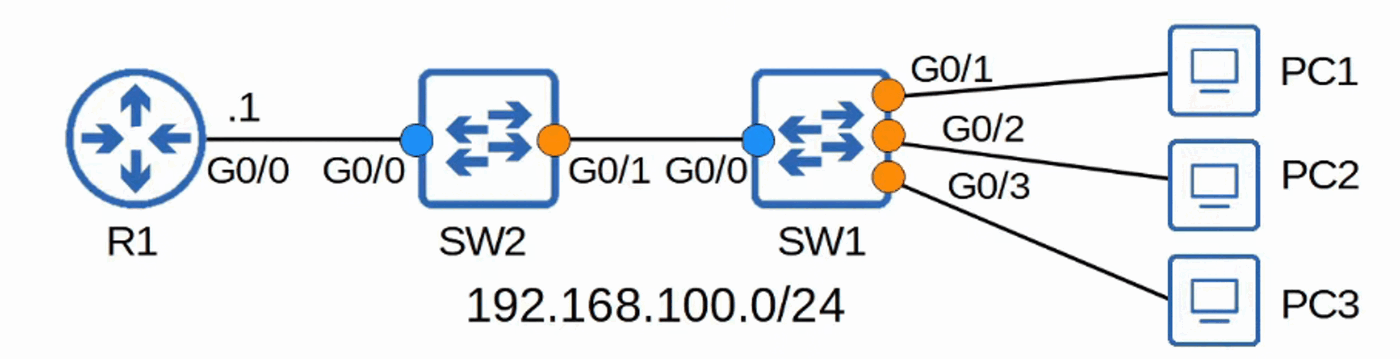
\includegraphics[keepaspectratio,alt={image}]{images/51-dhcp-snooping/img-006.png}}
\end{figure}

SWITCH 2's CONFIGURATION

\begin{figure}
\centering
\pandocbounded{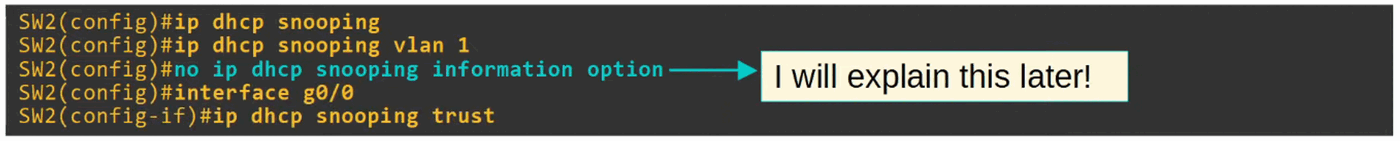
\includegraphics[keepaspectratio,alt={image}]{images/51-dhcp-snooping/img-007.png}}
\end{figure}

SWITCH 1's CONFIGURATION

\begin{figure}
\centering
\pandocbounded{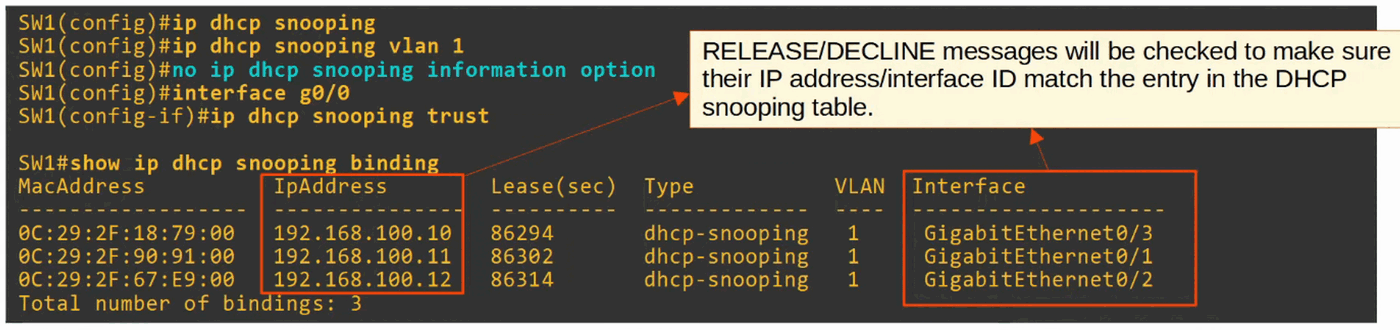
\includegraphics[keepaspectratio,alt={image}]{images/51-dhcp-snooping/img-008.png}}
\end{figure}

\section{DHCP Snooping Rate-Limiting}\label{dhcp-snooping-rate-limiting}

\begin{itemize}
\tightlist
\item
  DHCP SNOOPING can limit the RATE at which DHCP messages are allowed to
  enter an INTERFACE
\item
  If the RATE of DHCP messages crosses the configured LIMIT, the
  INTERFACE is \passthrough{\lstinline!err-disabled!}
\item
  Like with PORT SECURITY, the interface can be manually re-enabled, or
  automatically re-enabled with
  \passthrough{\lstinline!errdisable recovery!}
\end{itemize}

\begin{figure}
\centering
\pandocbounded{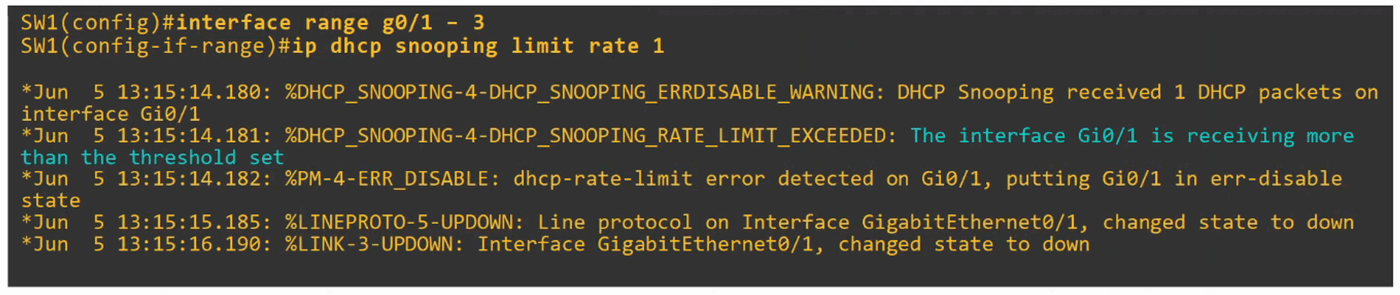
\includegraphics[keepaspectratio,alt={image}]{images/51-dhcp-snooping/img-009.png}}
\end{figure}

\begin{itemize}
\tightlist
\item
  You wouldn't set the limit rate to 1 since it's so low, it would shut
  the port immediately but this shows how RATE-LIMITING works
\end{itemize}

\passthrough{\lstinline!errdisable recovery cause dhcp-rate-limit!}

\begin{figure}
\centering
\pandocbounded{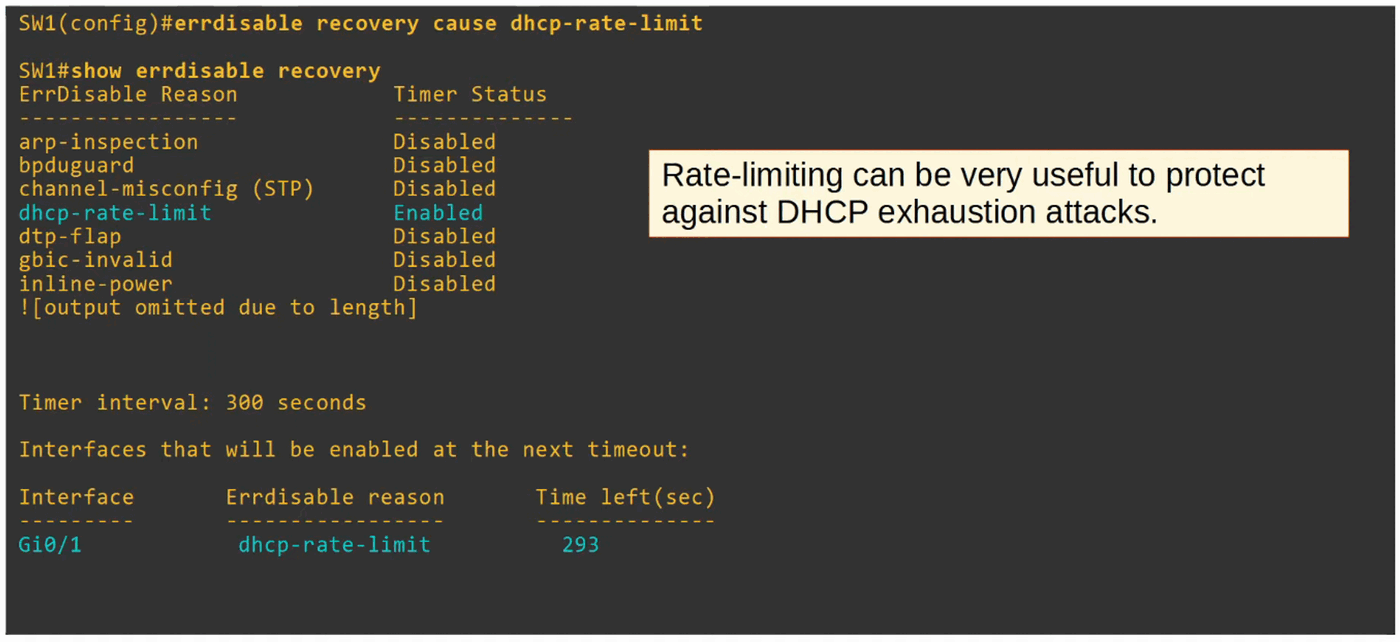
\includegraphics[keepaspectratio,alt={image}]{images/51-dhcp-snooping/img-010.png}}
\end{figure}

\section{DHCP Option 82 (Information
Option)}\label{dhcp-option-82-information-option}

\begin{itemize}
\tightlist
\item
  OPTION 82, also known as a `DHCP RELAY AGENT INFOMRATION OPTION' is
  one of MANY DHCP OPTIONS
\item
  It provides additional information about which DHCP RELAY AGENT
  received the CLIENT'S message, on which INTERFACE, in which VLAN, etc.
\item
  DHCP RELAY AGENTS can add OPTION 82 to message they forward to the
  remote DHCP SERVER
\item
  With DHCP SNOOPING enabled, by default Cisco SWITCHES will add OPTION
  82 to DHCP messages they receive from CLIENTS, even if the SWITCH
  isn't acting as a DHCP RELAY AGENT
\item
  By DEFAULT, Cisco SWITCHES will drop DHCP MESSAGES with OPTION 82 that
  are received on an UNTRUSTED PORT
\end{itemize}

\begin{figure}
\centering
\pandocbounded{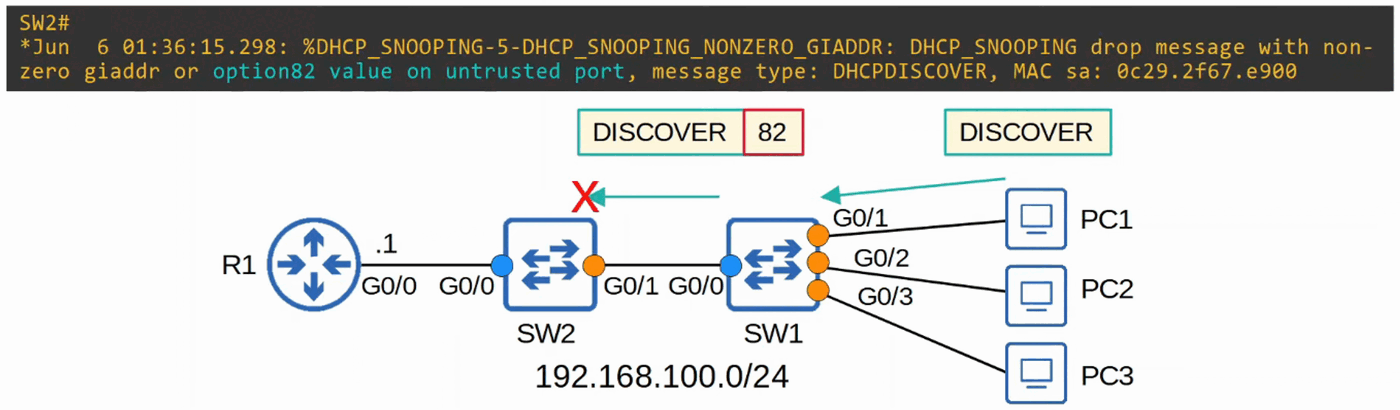
\includegraphics[keepaspectratio,alt={image}]{images/51-dhcp-snooping/img-011.png}}
\end{figure}

THIS command disables OPTION 82 for SW1 but NOT SW2

\begin{figure}
\centering
\pandocbounded{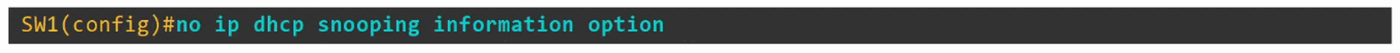
\includegraphics[keepaspectratio,alt={image}]{images/51-dhcp-snooping/img-012.png}}
\end{figure}

TRAFFIC gets passed to R1 and is DROPPED because of ``inconsistent relay
information'' (packet contains OPTION 82 but wasn't dropped by SW2)

\begin{figure}
\centering
\pandocbounded{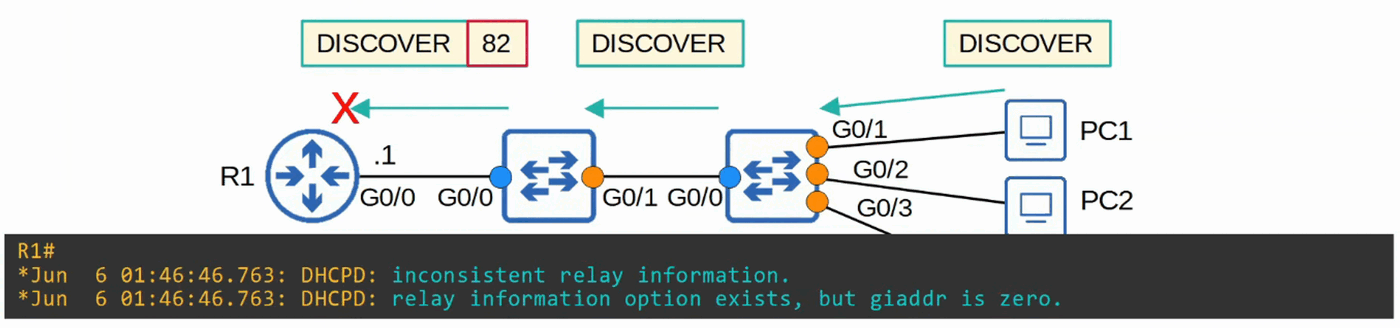
\includegraphics[keepaspectratio,alt={image}]{images/51-dhcp-snooping/img-013.png}}
\end{figure}

By ENABLING OPTION 82 on both SWITCHES\ldots{}

\begin{figure}
\centering
\pandocbounded{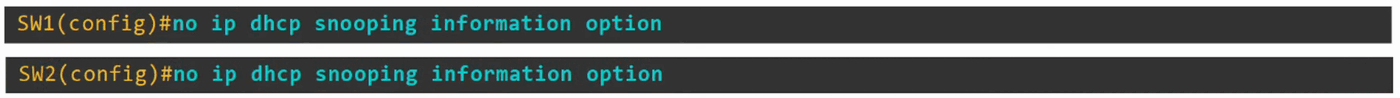
\includegraphics[keepaspectratio,alt={image}]{images/51-dhcp-snooping/img-014.png}}
\end{figure}

PC1's DHCP DISCOVER message gets passed, through SW1 and SW2, to R1. R1
responds with an DHCP OFFER message, as normal

\begin{figure}
\centering
\pandocbounded{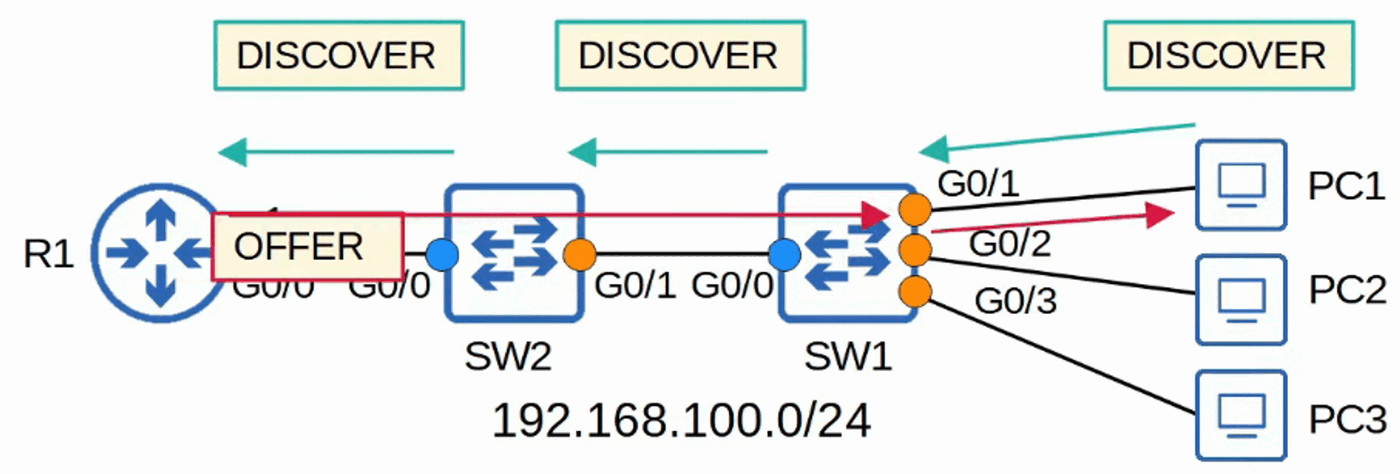
\includegraphics[keepaspectratio,alt={image}]{images/51-dhcp-snooping/img-015.png}}
\end{figure}

\section{Command Summary}\label{command-summary}

\begin{figure}
\centering
\pandocbounded{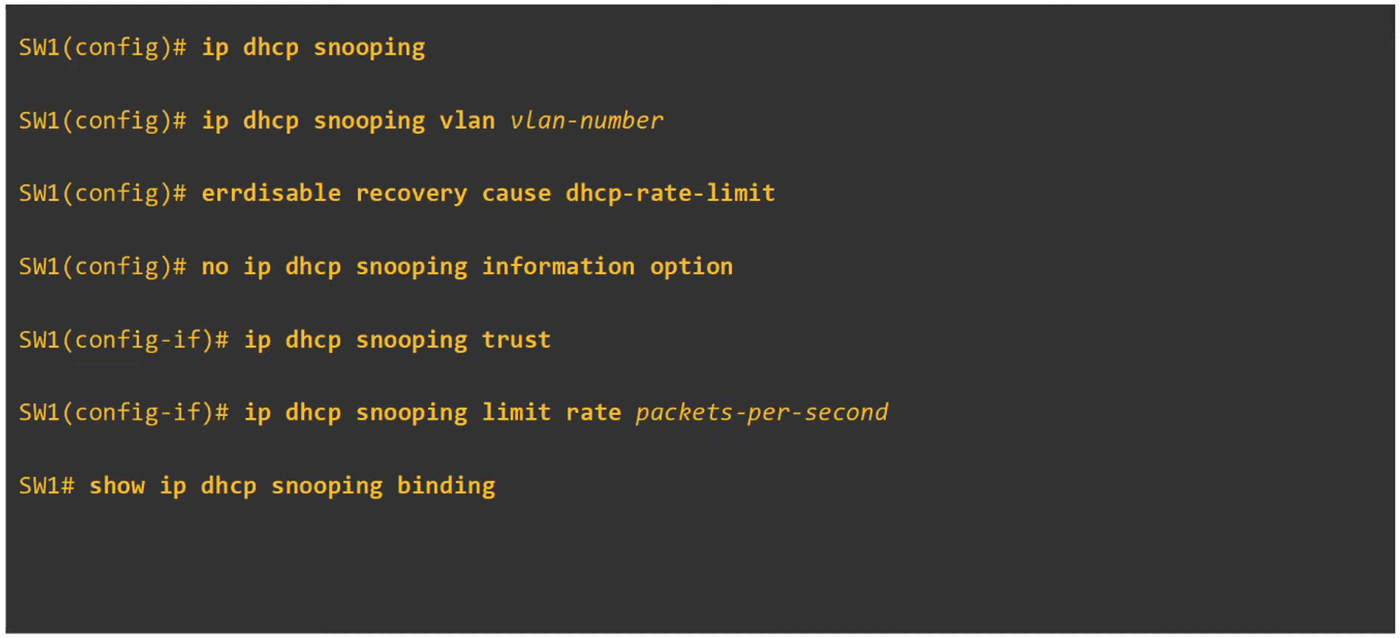
\includegraphics[keepaspectratio,alt={image}]{images/51-dhcp-snooping/img-016.png}}
\end{figure}
